\documentclass{bioinfo}
\copyrightyear{2012}
\pubyear{2012}

\begin{document}
\firstpage{1}

\title[Scythe]{Scythe: A tool for removing 3'-end adapter contaminants using Bayesian classification}
\author[Buffalo \textit{et~al}]{Vince Buffalo\,\footnote{to whom correspondence should be addressed}, Joseph Fass\, and Dawei Lin}
\address{Bioinformatics Core, UC Davis Genome Center}

\history{Received on XXXXX; revised on XXXXX; accepted on XXXXX}

\editor{Associate Editor: XXXXXXX}

\maketitle

\begin{abstract}

\section{Motivation:}
Modern sequencing technologies can leave artifactual contaminant
sequences at the 3'-end of reads. 3'-end regions also have the lowest
quality bases that are likely to be called incorrectly, which makes
identifying and removing 3'-end contaminants difficult. 

\section{Results:} 
Scythe is a program designed specifically to remove 3'-end
contaminants. It searches for 3'-end contaminants and uses a Bayesian
model that considers individual base qualities to decide whether a
given match is a contaminant or background sequence. With a variety of
contamination rates, Scythe outperforms other adapter removal software
tools.

\section{Availability:}
Scythe is freely available under the MIT license at
\href{http://github.com/vsbuffalo/scythe}{http://github.com/vsbuffalo/scythe}.

\section{Contact:} \href{mailto:vsbuffalo@gmail.com}{vsbuffalo@gmail.com}
\end{abstract}

\section{Introduction}
Scythe is focused on trimming 3'-end contaminants, specifically those
due to adapters or barcodes. It embraces the Unix Philosophy of
``programs that do one thing well'' (\citealp{raymond2003}). Many
second-generation sequencing technologies such as Illumina's Genome
Analyzer II and HiSeq have lower-quality 3'-end bases. These
low-quality bases are more likely to have nucleotides called
incorrectly, making contaminant identification more
difficult. Futhermore, 3'-end quality deterioration is not uniform
across all reads (see Fig. 1 in Supplementary Materials).

By using a Bayesian classification procedure, Scythe accurately trims
3'-end contaminants off reads. The underlying model differentially
weights mismatching bases according to their FASTQ quality.

% A common step in read quality improvement procedures is to remove
% these low-quality 3'-end sequences from reads. This is thought to
% increase mapping rates and improve assembly quality. However doing
% quality-based 3'-end trimming before contaminant removal would remove
% sequence that could be used (despite being unreliable) to identify the
% contaminants more accurately. Scythe takes the approach that it is
% better to use full information, even if it's unreliable. How
% unreliable a base is is indicated by the FASTQ quality score, which
% can be incorporated into Scythe's classification procedure.

% Fixed-number of mismatch approaches have the disadvantage that they
% do not differentially weight a mismatch on a low-quality base from a
% mismatch on a high-quality base. Futhermore, the fixed-number could
% easily be exhausted in a run of bad bases (which are quite common in
% the 3'-end), even though every good-quality base perfectly matches the
% contaminant sequence.


\begin{methods}
\section{String Matching in Scythe}

Scythe employs a simple string matching heuristic to find a best
match. Scythe scores each alignment of the contaminant sequence
against the read sequence, starting from the entire contaminant in the
3'-end to incrementally fewer bases. A minimum match length can be
specified via a parameter (by default, 5). Each of these alignments is
scored using a $1$ for match, $-1$ for mismatch approach. The top
scoring alignment is then passed to the probabilistic classification
procedure, which decides whether the match is background sequence or a
contaminant. The time complexity of Scythe's matching algorithm for a
single adapter of length $l_a$ is $O(l_a^2 R)$ for a FASTQ file with
$R$ entries.


\section{Bayesian Classification of Top-Scoring Matches}

There are two mutually exclusive and exhaustive events: a top scoring
match is a contaminant or it is random sequence (that happens to be
similar to the adapter contaminant). A likelihood for each of these
events, given probabilities of each base being called correctly and
which bases mismatch the contaminant sequence, can be calculated.

These likelihood functions assume models of error for each event. If
the top-scoring match is contaminant sequence (event $C$), the
likelihood $P(S | C)$ (where $S$ is the sequence match data) is:

$$ P(S | C) = \prod_{i=1}^{l_t} q_i^{m_i} \cdot (1-q_i)^{1 - m_i} $$

Where $m_i \in \{0, 1\}$ indicating whether the $i$ base is a mismatch
or match (respectively) and $q_i$ is the probability the $i$ base is
called correctly (from the ASCII-encoded quality). $l_t$ is the length
of the top-scoring match.

If the top-scoring sequence is not a contaminant sequence (event
$C'$), it is assumed that the matches are just by chance. Thus, the
likelihood function is:

$$ P(S | C') = \prod_{i=1}^{l_t} \left(\frac{1}{4}\right)^{m_i} \cdot \left(\frac{3}{4}\right)^{1 - m_i} $$

These likelihoods can then be combined using Bayes' Thereom to give
the probability of contamination given the top-scoring match:

$$ P(C|S) = \frac{P(C) P(S|C)}{P(S)} $$

Since these are mutually exclusive and exhaustive events, the
\emph{maximum a posteriori} rule can be used to classify a top-scoring
sequence as either contaminated or non-contaminated (e.g. if $P(C'|S)
> P(C|S)$, the sequence is not contaminated and visa-versa).

Required in this Bayesian formulation is the prior of contamination,
$P(C)$. Specifying the prior may seem like a nuisance, but it is a
useful parameter that can be adjusted for a variety of different
contamination scenarios. More information on specifying a parameter is
in Supplementary Materials.

\section{Results}
\begin{centering}
\begin{figure*}[!tpb]
\includegraphics[angle=-90]{graphics/roc-and-incorrect-trimmed.eps}
\caption{ROC curve showing Scythe's higher rate of true positives for
  a given false positive rate and a bar chart indicating Scythe's
  fewer incorrectly trimmed reads.}\label{fig:02}
\end{figure*}
\end{centering}

Scythe was tested against two similar program: Btrim
(\citealp{pmid21651976}) and Cutadapt (\citealp{EJ200}). Both
Btrim and Cutadapt can handle insertions/deletions, but in Illumina
data we've analzed, no indels in adapter contaminants were
witnessed. This problem is more associated with 454 reads, which can
have homopolymer repeats. Both Btrim and Cutadapt also include quality
trimmers, which Scythe intentionally does not.

To test Scythe, Btrim, and Cutadapt at 3'-end adapter contaminant
removal, random reads were generated and contaminated at fixed
contamination rates of 40\% and 70\%. FASTQ qualities from an Illumina
HiSeq run were added to these read sequences. Real base qualities were
used because properly modeling and simulating 3'-end quality
degradation is an arduous task. For the two fixed contamination rates,
ten replicate FASTQ files were generated randomly to ensure
contaminated and non-contaminated reads were well dispersed across
different read qualities. Each simulated FASTQ reads file contains
10,000 entries.

Each program was run with varying parameters to see how true positive
and false positive rates change. Btrim uses a fixed number of
mismatches, so integer values from 0 to 10 were used. Cutadapt uses an
error rate for a matched sequence, which was varied from 0 to 0.95 in
0.05 increments. Likewise, Scythe uses the same values for its prior
parameter. Each piece of software was run with all other options off
to ensure a fair comparison of 3'-end contaminant removal.

While Cutadapt and Scythe only trim reads, Btrim occasionally removes
a read entirely from the sample. For comparison purposes, we count
this as trimming the entire length of a read. We compared the length
of the original simulated read to the trimmed read for all programs,
parameters, replicates, and contamination rates. This, combined with
information about whether a read was contaminated allows the
calculation of true positive and false positive rates. Also, we
investigate how many times Btrim, Cutadapt, and Scythe incorrectly
trim a read, e.g. whether the trimmed length is not equal to the
contaminate length for reads that were contaminated.

In these tests, we find that Scythe outperforms Btrim and Cutadapt in
terms of true positive rates for a variety of false positive rates
across a variety of parameters (Fig. \ref{fig:02}). Furthermore,
Scythe also has fewer incorrectly trimmed reads across a variety of
parameters compared to Btrim and Cutadapt. Differences in
contamination rates (40\% and 70\%) do not adversely affect Scythe's
performance. Note that Cutadapt performs well too, but is very
sensitive to its error parameter. Changing Cutadapt's error parameter
from 35\% to 40\% slightly increases the true positive rate, but
drastically increases the false positive rate. By contrast, Scythe's
probabilistic approach is much less sensitive to different prior
parameters, illustrated by the overplotting of the 35\% to 95\% prior
parameters in the ROC curve (Fig. \ref{fig:02}). Furthermore, we argue
that Scythe's parameter is easier to intuitively choose than a
sequence error rate.

\end{methods}

\section{Conclusion}

When compared to Btrim and Cutadapt, Scythe is a very accurate 3'-end
contaminant trimmer appropriate for a variety of pre-analysis quality
pipelines. It is a modular and orthogonal program, allowing use with
other read processing tools and diagnostics between each step. We
suggest that Scythe be used for all Illumina read processing
pipelines.

We suspect Scythe's superior performance is due to its (1)
consideration of base-level qualities and (2) Scythe's use of Bayesian
model rather than a simple fixed-number of mismatches or fixed-error
approach.


\section*{Acknowledgement}
Monica Britton and Nikhil Joshi for helpful feedback about bugs in
Scythe. Xiran Dong was very helpful in early testing of Scythe against
other trimmers.

%\paragraph{Funding\textcolon} None.


\bibliographystyle{natbib}
% \bibliographystyle{achemnat}
% \bibliographystyle{plainnat}
% \bibliographystyle{abbrv}
% \bibliographystyle{bioinformatics}
\nocite{qrqc}
\nocite{ShortRead}
\nocite{Biostrings}
\nocite{ggplot2}

\bibliography{references}


\end{document}
